\section{El DUNE verso: módulos}

\begin{frame}[fragile]
	\frametitle{\secname}
	\framesubtitle{\url{https://dune-project.org/groups/core}}

	\begin{figure}[ht!]
		\centering
		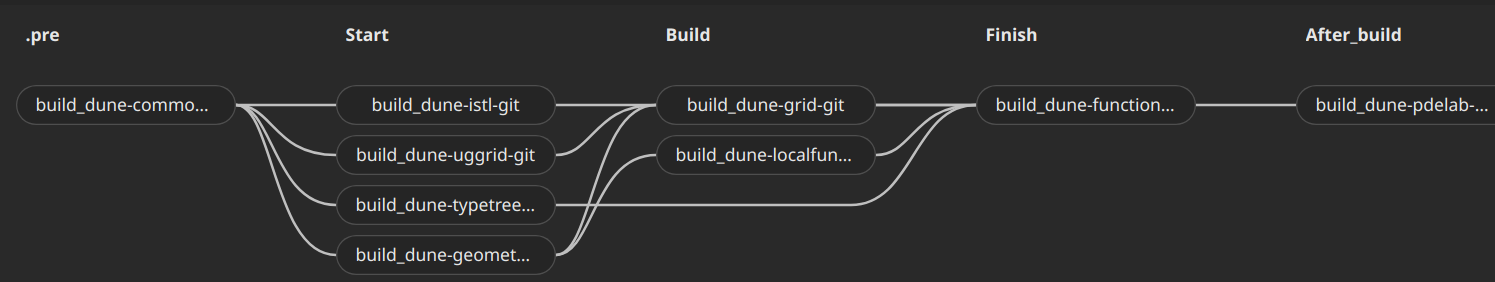
\includegraphics[width=14.6cm]{dependences}
		\caption{Tomado de \url{https://gitlab.com/dune-archiso/repository/dune-archiso-repository-pdelab-git/-/pipelines}}
	\end{figure}

	\begin{description}
		\item[dune-common]

			Clases fundamentales e infraestructura para la construcción del sistema.

		\item[dune-geometry]

			Elementos de referencia, métodos de cuadratura y transformaciones geométricas.

		\item[dune-grid]

			Interfaces con las mallas (ALUGrid, UGGrid, Alberta, YasGrid), construcción y visualización.

		\item[dune-istl]

			Biblioteca de solucionadores iterativas de plantillas, clases genéricas de matrices/vectores dispersos, solucionadores

		\item[dune-localfunctions]

			Interface genérica para funciones de elementos finitos.
	\end{description}

	\note{
		\begin{description}
			\item[dune-common]
				Contiene las clases base usadas por todos los módulos de DUNE-modules.

				Provee algunas clases de infraestructura para depuración y manejo de excepciones así como una librería para manejar una matriz densa y vectores.

			\item[dune-grid]
				Define mallas jerarquizadas, paralelas, de dimensiones arbitrarias, permite salida a formatos que puedens ser leídos por ParaView.
		\end{description}
	}
\end{frame}

\subsection{Dependencias de algunos módulos}

\begin{frame}
	\frametitle{\secname}
	\framesubtitle{\subsecname}

	\begin{columns}
		\begin{column}{0.5\textwidth}
			\dirtree{%
				.1 dune-fem.
				.2 dune-grid.
				.3 dune-geometry.
				.4 dune-common.
			}

			\

			\

			\dirtree{%
				.1 dumux.
				.2 dune-istl.
				.2 dune-localfunctions.
				.2 vc.
				.2 psurface.
				.2 superlu.
				.2 arpack++.
				.2 suitesparse.
				.2 dune-alugrid.
				.2 dune-subgrid.
				.2 fmt.
				.2 opm-common.
			}
		\end{column}

		\begin{column}{0.5\textwidth}
			\dirtree{%
				.1 opm-upscaling.
				.2 opm-grid.
				.3 opm-common.
				.4 dune-grid.
				.5 dune-geometry.
				.4 dune-istl.
				.4 boost.
			}

			\

			\

			\dirtree{%
				.1 opm-models.
				.2 opm-material.
				.3 opm-common.
				.4 dune-grid.
				.5 dune-geometry.
				.4 dune-istl.
				.4 boost.
			}
		\end{column}
	\end{columns}

	\note{
		Aquí se puede ver la relación de dependencias entre los módulos de DUNE.
	}

\end{frame}